\shorthandoff{<>}
\begin{tikzpicture}[font=\small]
    \draw[draw=black, fill=gray!15, thick] (0,0) ellipse (1.25 and 0.85);
    \node at (0,0.18) {objeto};
    \node at (0,-0.23) {$f(x)$};

    \draw[fill=black!10, draw=black, thick] (-4,0.55) -- (-3.35,0.9) -- (-3.35,0.2) -- cycle;
    \draw[fill=black!35, draw=black] (-4.25,0.42) rectangle (-4,0.68);
    \node[above] at (-3.75,0.92) {fuente};

    \draw[thick] (3.45,-1.45) -- (3.45,1.45);
    \foreach \y in {-1.25,-0.85,...,1.15} {
        \draw[thin] (3.35,\y) -- (3.55,\y);
    }
    \node[right] at (3.55,0) {detector};

    \draw[densely dashed, thin, gray] (-3.25,0.55) -- (3.35,1.15);
    \draw[densely dashed, thin, gray] (-3.25,0.55) -- (3.35,-0.35);
    \draw[->, thick] (-3.25,0.55) -- (3.35,0.55) node[pos=0.20, above] {$I_0$} node[pos=0.86, above] {$I$};
    \node[above] at (0,0.62) {trayectoria $\gamma$};

    \node[align=center, below] at (0,-1.45)
    {$-\log\!\left(\dfrac{I}{I_0}\right)=\displaystyle\int_\gamma f(x)\,ds$};
\end{tikzpicture}
\shorthandon{<>}
